\documentclass[a4paper, 12pt]{article}
\usepackage[a4paper,top=1.5cm, bottom=1.5cm, left=1cm, right=1cm]{geometry}
\usepackage{cmap}					
\usepackage{mathtext} 				
\usepackage[T2A]{fontenc}			
\usepackage[utf8]{inputenc}			
\usepackage[english,russian]{babel}
\usepackage{multirow}
\usepackage{graphicx}
\usepackage{wrapfig}
\usepackage{tabularx}
\usepackage{float}
\usepackage{longtable}
\usepackage{hyperref}
\hypersetup{colorlinks=true,urlcolor=blue}
\usepackage[rgb]{xcolor}
\usepackage{amsmath,amsfonts,amssymb,amsthm,mathtools} 
\usepackage{icomma} 
\usepackage{euscript}
\usepackage{mathrsfs}
\usepackage{enumerate}
\usepackage{caption}
\usepackage{enumerate}
\mathtoolsset{showonlyrefs=true}
\usepackage{graphicx}
\usepackage{caption}
\usepackage{subcaption}
\usepackage[europeanresistors, americaninductors]{circuitikz}
\DeclareMathOperator{\sgn}{\mathop{sgn}}
\newcommand*{\hm}[1]{#1\nobreak\discretionary{}
	{\hbox{$\mathsurround=0pt #1$}}{}}

\title{\textbf{Измерение вязкости воздуха по течению в тонких трубках (1.3.3)}}
\author{Ладченко Мария}
\date{}

\begin{document}

\maketitle
	      	
    \begin{center}
    \section*{Введение}    
    \end{center}

    \noindent \textbf{Цель работы:} экспериментально исследовать свойства течения газов по тонким трубкам при различных числах Рейнольдса; выявить область применимости закона Пуазейля и с его помощью определить коэффициент вязкости воздуха.

    \bigskip

    \noindent \textbf{Оборудование:} система подачи воздуха (компрессор, поводящие трубки); газовый счетчик барабанного типа; спиртовой микроманометр с регулируемым наклоном; набор трубок различного диаметра с выходами для подсоединения микроманометра; секундомер.
    \bigskip

\begin{center}
\subsection*{Теоретические сведения}    
\end{center}

Рассмотрим движение вязкой жидкости или газа по трубке круглого сечения. При малых скоростях потока движение оказывается ламинарным (слоистым), скорости частиц меняются по радиусу и направлены вдоль оси трубки. С увеличением скорости потока движение становится турбулентным, а слои перемешиваются. При турбулентном движении скорость в каждой точке быстро меняет величину и направление, сохраняется только средняя величина скорости.

Характер движения газа (или жидкости) в трубке определяется безразмерным числом Рейнольдса:
\[
	Re = \frac{vr\rho}{\eta}
\]
где $v$ -- скорость потока, $r$ -- радиус трубки, $\rho$ -- плотность движущейся среды, $\eta$ -- её вязкость. В гладких трубах круглого сечения переход от ламининарного движения к турбулентному происходит при $Re \approx 1000$.

При ламинарном течении объем газа $V$, протекающий за время $t$ по трубе длиной $l$, определяется формулой Пуазейля:
\begin{equation}
	Q = \frac{\pi r^4}{8 \Delta l \eta}(P_1 - P_2)
\end{equation}
В этой формуле $P_1 - P_2$ -- разность давлений в двух выбранных сечениях 1 и 2, расстояние между которыми равно $\Delta l$. Величину $Q$ обычно называют расходом. Формула (1) позволяет определять вязкость газа по его расходу.

Отметим условия, при которых справедлива формула (1). Прежде всего необходимо, чтобы с достаточным запасом выполнялось неравенство $Re < 1000$. Необходимо также, чтобы при течении не происходило существенного изменения удельного объёма газа (при выводе формулы удельный объём считался постоянным). Для жидкости это предположение выполняется практически всегда, а для газа --- лишь в тех случаях, когда перепад давлений вдоль трубки мал по сравнению с самим давлением. В нашем случае давление газа равно атмосферному ($10^3$ см вод. ст.), а перепад давлений составляет не более 10 см вод. ст., т. е. менее 1\% от атмосферного. Формула (1) выводится для участков трубки, на которых закон распределения скоростей газа по сечению не меняется при двидении вдоль потока.
\begin{figure}[H]
\center
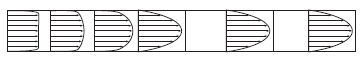
\includegraphics[scale=1]{potok.png}
\caption{Формирование потока газа в трубке круглого сечения}
\end{figure}
При втекании газа в трубку из большого резервуара скорости слоёв вначале постоянны по всему направлению. По мере продвижения газа по трубке картина распределения скоростей меняется, так как сила трения о стенку тормозит прилежащие к ней оси. Характерное для ламинарного течения параболическое распределение скоростей устанавливается на некотором расстоянии $a$ от входа в трубку, которое зависит от радиуса трубки $r$ и числа Рейнольдса по формуле 
\begin{equation}
	a \approx 0.2rRe
\end{equation}
Градиент давления на участке формирования потока оказывается больше, чем на участке с установившимся ламинарным течением, что позволяет разделить эти участки экспериментально. Формула (2) даёт возможность оценить дину участка формирования.

\begin{center}
\subsection*{Экспериментальная установка}    
\end{center}

Схема экспериментальной установки изображена на Рис. \ref{233}. Поток воздуха
под давлением, немного превышающим атмосферное, поступает через газовый счётчик в тонкие металлические трубки. Воздух нагнетается компрессором, интенсивность его подачи регулируется краном К. Трубки снабжены
съёмными заглушками на концах и рядом миллиметровых отверстий, к которым можно подключать микроманометр. В рабочем состоянии открыта заглушка на одной (рабочей) трубке, микроманометр подключён к двум её выводам, а все остальные отверстия плотно закрыты пробками.

\begin{figure}[H]
    \centering
    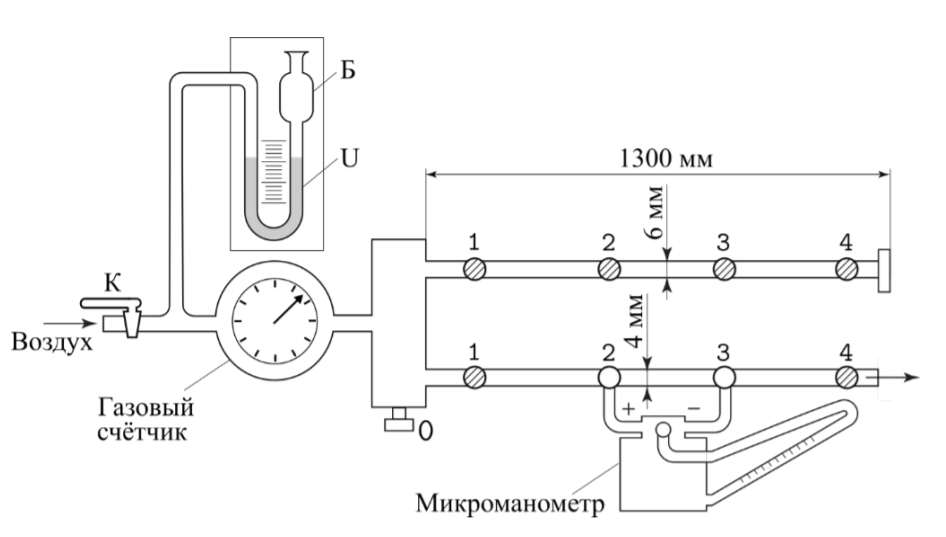
\includegraphics[scale=0.65]{expust.PNG}
    \caption{Экспериментальная установка}
    \label{233}
\end{figure}

Перед входом в газовый счётчик установлен водяной U-образный манометр. Он служит для измерения давления газа на входе, а также предохраняет
счётчик от выхода из строя. При превышении максимального избыточного
давления на входе счётчика ($\sim$ 30 см вод. ст.) вода выплёскивается из трубки
в защитный баллон Б, создавая шум и привлекая к себе внимание экспериментатора.


\textbf{Газовый счётчик.} В работе используется газовый счётчик барабанного
типа, позволяющий измерять объём газа $\Delta V$ прошедшего через систему. Измеряя время $\Delta t$ при помощи секундомера, можно вычислить средний объёмный расход газа $Q = \Delta V/ \Delta t$ (для получения массового расхода [кг/с] результат
необходимо домножить на плотность газа $\rho$).

\begin{figure}[H]
    \centering
    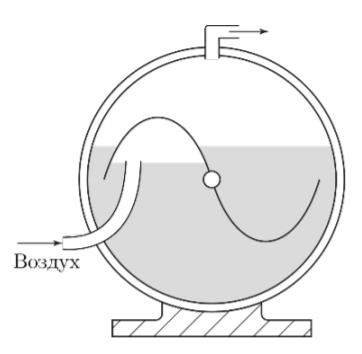
\includegraphics[scale=0.65]{gascounter.PNG}
    \caption{Газовый счетчик}
    \label{333}
\end{figure}


Работа счётчика основана на принципе вытеснения: на цилиндрической ёмкости жёстко
укреплены лёгкие чаши (см. Рис. \ref{333}, где для
упрощения изображены только две чаши), в которые поочередно поступает воздух из входной
трубки расходомера. Когда чаша наполняется,
она всплывает и её место занимает следующая
и т.д. Вращение оси предаётся на счётно-суммирующее устройство.
Для корректной работы счётчика он должен
быть заполнен водой и установлен горизонтально по уровню (подробнее см. техническое
описание установки).

\textbf{Микроманометр.} В работе используется жидкостный манометр с наклонной трубкой. Разность давлений на входах манометра измеряется по высоте
подъёма этилового спирта. Регулировка
наклона позволяет измерять давление в различных диапазонах.

На крышке прибора установлен трехходовой кран, имеющий два рабочих
положения — (0) и (+). В положении (0) производится установка мениска жидкости на ноль, что необходимо сделать перед началом работы (в процессе работы также рекомендуется периодически проверять положение нуля). В положении (+) производятся измерения.
\newpage

\begin{center}
    
    \section*{Ход работы}

    Эксперимент проводился при комнатной температуре $T_\text{комн}=298,6 K$, при атмофсерном давлении $P_\text{атм}=101,75$ кПа и при относительной влажности в помещении $\eta=74\%$.

Давление, измеряемое микроманометром, определяется по формуле:
\[
P=9,81 \cdot K \cdot l 
\]
где $l$ -- показание макроманометра, $K$ -- коэффициент наклона, $P$ -- Давление в паскалях.

\subsection*{Зависимость разности давлений от расхода}

Эксперимент проводился на первой трубе с диаметром $d_1=4,10\pm0,05$ мм.
    
    
    \begin{table}[h]
        \centering
        \begin{tabular}{|c|c|c|c|c|}
    
            
            \hline \hline
            $\varDelta P, \text{дел}$ & $V, \text{л}$ & $\varDelta P, \text{Па}$ & $Q, \text{л}/\text{с}}$ & $\varDelta t, \text{с}$ \\ \hline
            241 & 4.807 & 472.84 & 160.23 & 30   \\ \hline
            215 & 4.518 & 421.83 & 150.60 & 30   \\ \hline
            189 & 4.209 & 370.81 & 140.30 & 30   \\ \hline
            171 & 3.979 & 335.50 & 132.63 & 30   \\ \hline
            149 & 3.755 & 292.33 & 125.16 & 30   \\ \hline
            130 & 3.549 & 255.06 & 118.30 & 30   \\ \hline
            102 & 3.205 & 200.12 & 106.83 & 30    \\ \hline
            94 & 3.118  & 184.42 & 103.93 & 30   \\ \hline
            89 & 3.063  & 174.61 & 102.10 & 30   \\ \hline
            84 & 2.971  & 164.80 & 99.03  & 30   \\ \hline
            77 & 2.899  & 151.07 & 96.63  & 30   \\ \hline
            71 & 2.787  & 139.30 & 92.90  & 30   \\ \hline
            66 & 2.626  & 129.49 & 87.53  & 30   \\ \hline
            61 & 2.450  & 119.68 & 81.66  & 30   \\ \hline
            55 & 2.222  & 107.91 & 74.06  & 30   \\ \hline
            50 & 2.050  & 98.10  & 68.33  & 30   \\ \hline
            45 & 1.868  & 88.29  & 62.26  & 30   \\ \hline
            39 & 1.623  & 76.51  & 54.1   & 30   \\ \hline
            34 & 1.433  & 66.70  & 47.76  & 30   \\ \hline
            30 & 1.252  & 58.86  & 41.73  & 30   \\ \hline
            25 & 1.059  & 49.05  & 35.29  & 30   \\ \hline
            20 & 0.841  & 39.24  & 28.03  & 30   \\ \hline
            \hline
        \end{tabular}
        
    \end{table}
\end{center}

По угловому коэффициенту и формуле (1) можно оценить вязкость воздуха, воспользовавшись МНК аппроксимацией. Она составила 
$\eta = (2,13 \pm 0,12) \cdot 10^{-5}$ Па$\cdot$с

\begin{figure}[H]
    \centering
    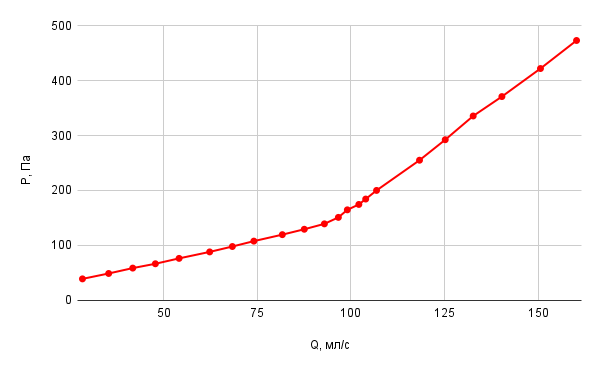
\includegraphics[scale=0.7]{chart1.png}
\end{figure}

Эксперимент проводился на второй трубе с диаметром $d_1=4,10\pm0,05$ мм., где $\varDelta t = 30 \text{с}$

\begin{table}[h]
    \centering
    \begin{tabular}{|c|c|c|c|c|}
    \hline
    \hline
    $\varDelta P, \text{Па}$ & $Q, \text{мл/c}$ \\ \hline
    274.68 & 259.16   \\ \hline
    233.47 & 239.53   \\ \hline
    196.20 & 212.73   \\ \hline
    184.42 & 199.63   \\ \hline
    176.58 & 190.53   \\ \hline
    166.77 & 184.26   \\ \hline
    156.96 & 177.66   \\ \hline
    145.18 & 174.30   \\ \hline
    137.34 & 171.46   \\ \hline
    123.60 & 160.53   \\ \hline
    105.94 & 156.53   \\ \hline
    68.67  & 153.93   \\ \hline 
    56.89  & 144.36   \\ \hline
    31.39  & 96.53    \\ \hline \hline
    \end{tabular}
\end{table}

По угловому коэффициенту и формуле (1) можно оценить вязкость воздуха, воспользовавшись МНК аппроксимацией. Она составила 
$\eta = (2,05 \pm 0,10q) \cdot 10^{-5}$ Па$\cdot$с

\begin{figure}[H]
    \centering
    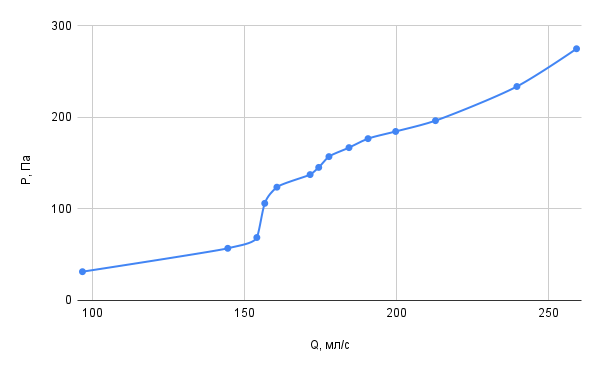
\includegraphics[scale=0.7]{chart2.png}
\end{figure}

\begin{center}
\subsection*{Зависимость разности давлений от длины участка}    
\end{center}

\begin{table}[h]
    \centering
    \begin{tabular}{|c|c|c|c|c|c|}
        \hline $ t$, с & $\Delta P$, Па & $L$, см & $Q$, мл/c\\
        \hline  30 & 321 & 131 & 69,6 \\
        \hline  30 & 221 & 81 & 69,9\\
        \hline 30 & 145 & 41  & 69,5\\
        \hline 30 & 68 & 11   & 60,7\\\hline       
    \end{tabular}
    \caption{Результаты измерений разности давлений от расхода}
    \label{p12}
\end{table}

\begin{figure}[H]
    \centering
    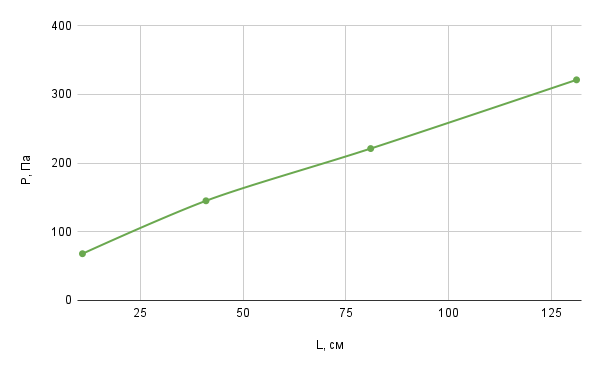
\includegraphics[scale=0.7]{chart3.png}
\end{figure}


\begin{center}
\begin{equation}
    Re_{\text{кр1}} = \frac{\rho Q}{\pi R \eta} = 902 \pm 48 \; \; \; \; \;
    Re_{\text{кр1}} = \frac{\rho Q}{\pi R \eta} = 1102 \pm 61
\end{equation}    
\end{center}


\begin{center}
    
    \section*{Вывод}
    экспериментально исследовать свойства течения газов по тонким трубкам при различных числах Рейнольдса; выявить область применимости закона Пуазейля и с его помощью определить коэффициент вязкости воздуха.
    
    \end{document}

\end{center}